\section{Marco Teorico}

\subsection{Redes Neuronales Graficas}

Las Redes Neuronales de grafos (GNN) son modelos de aprendizaje profundo en los cuales se procesan datos en representaciones de grafos o redes. Las GNN permiten aprovechar las relaciones que se codifican en los grafos para extraer características significativas y realizar tareas como la clasificación de nodos, la predicción de aristas (conexiones) y la inferencia a nivel de grafo. Este tipo de modelos aprende de las incrustaciones que capturen la informacion estructural del grafo como las características que se tengan en los nodos como se puede observar en la figura \ref{fig:GNN}

\begin{figure}[h!]
    \centering
    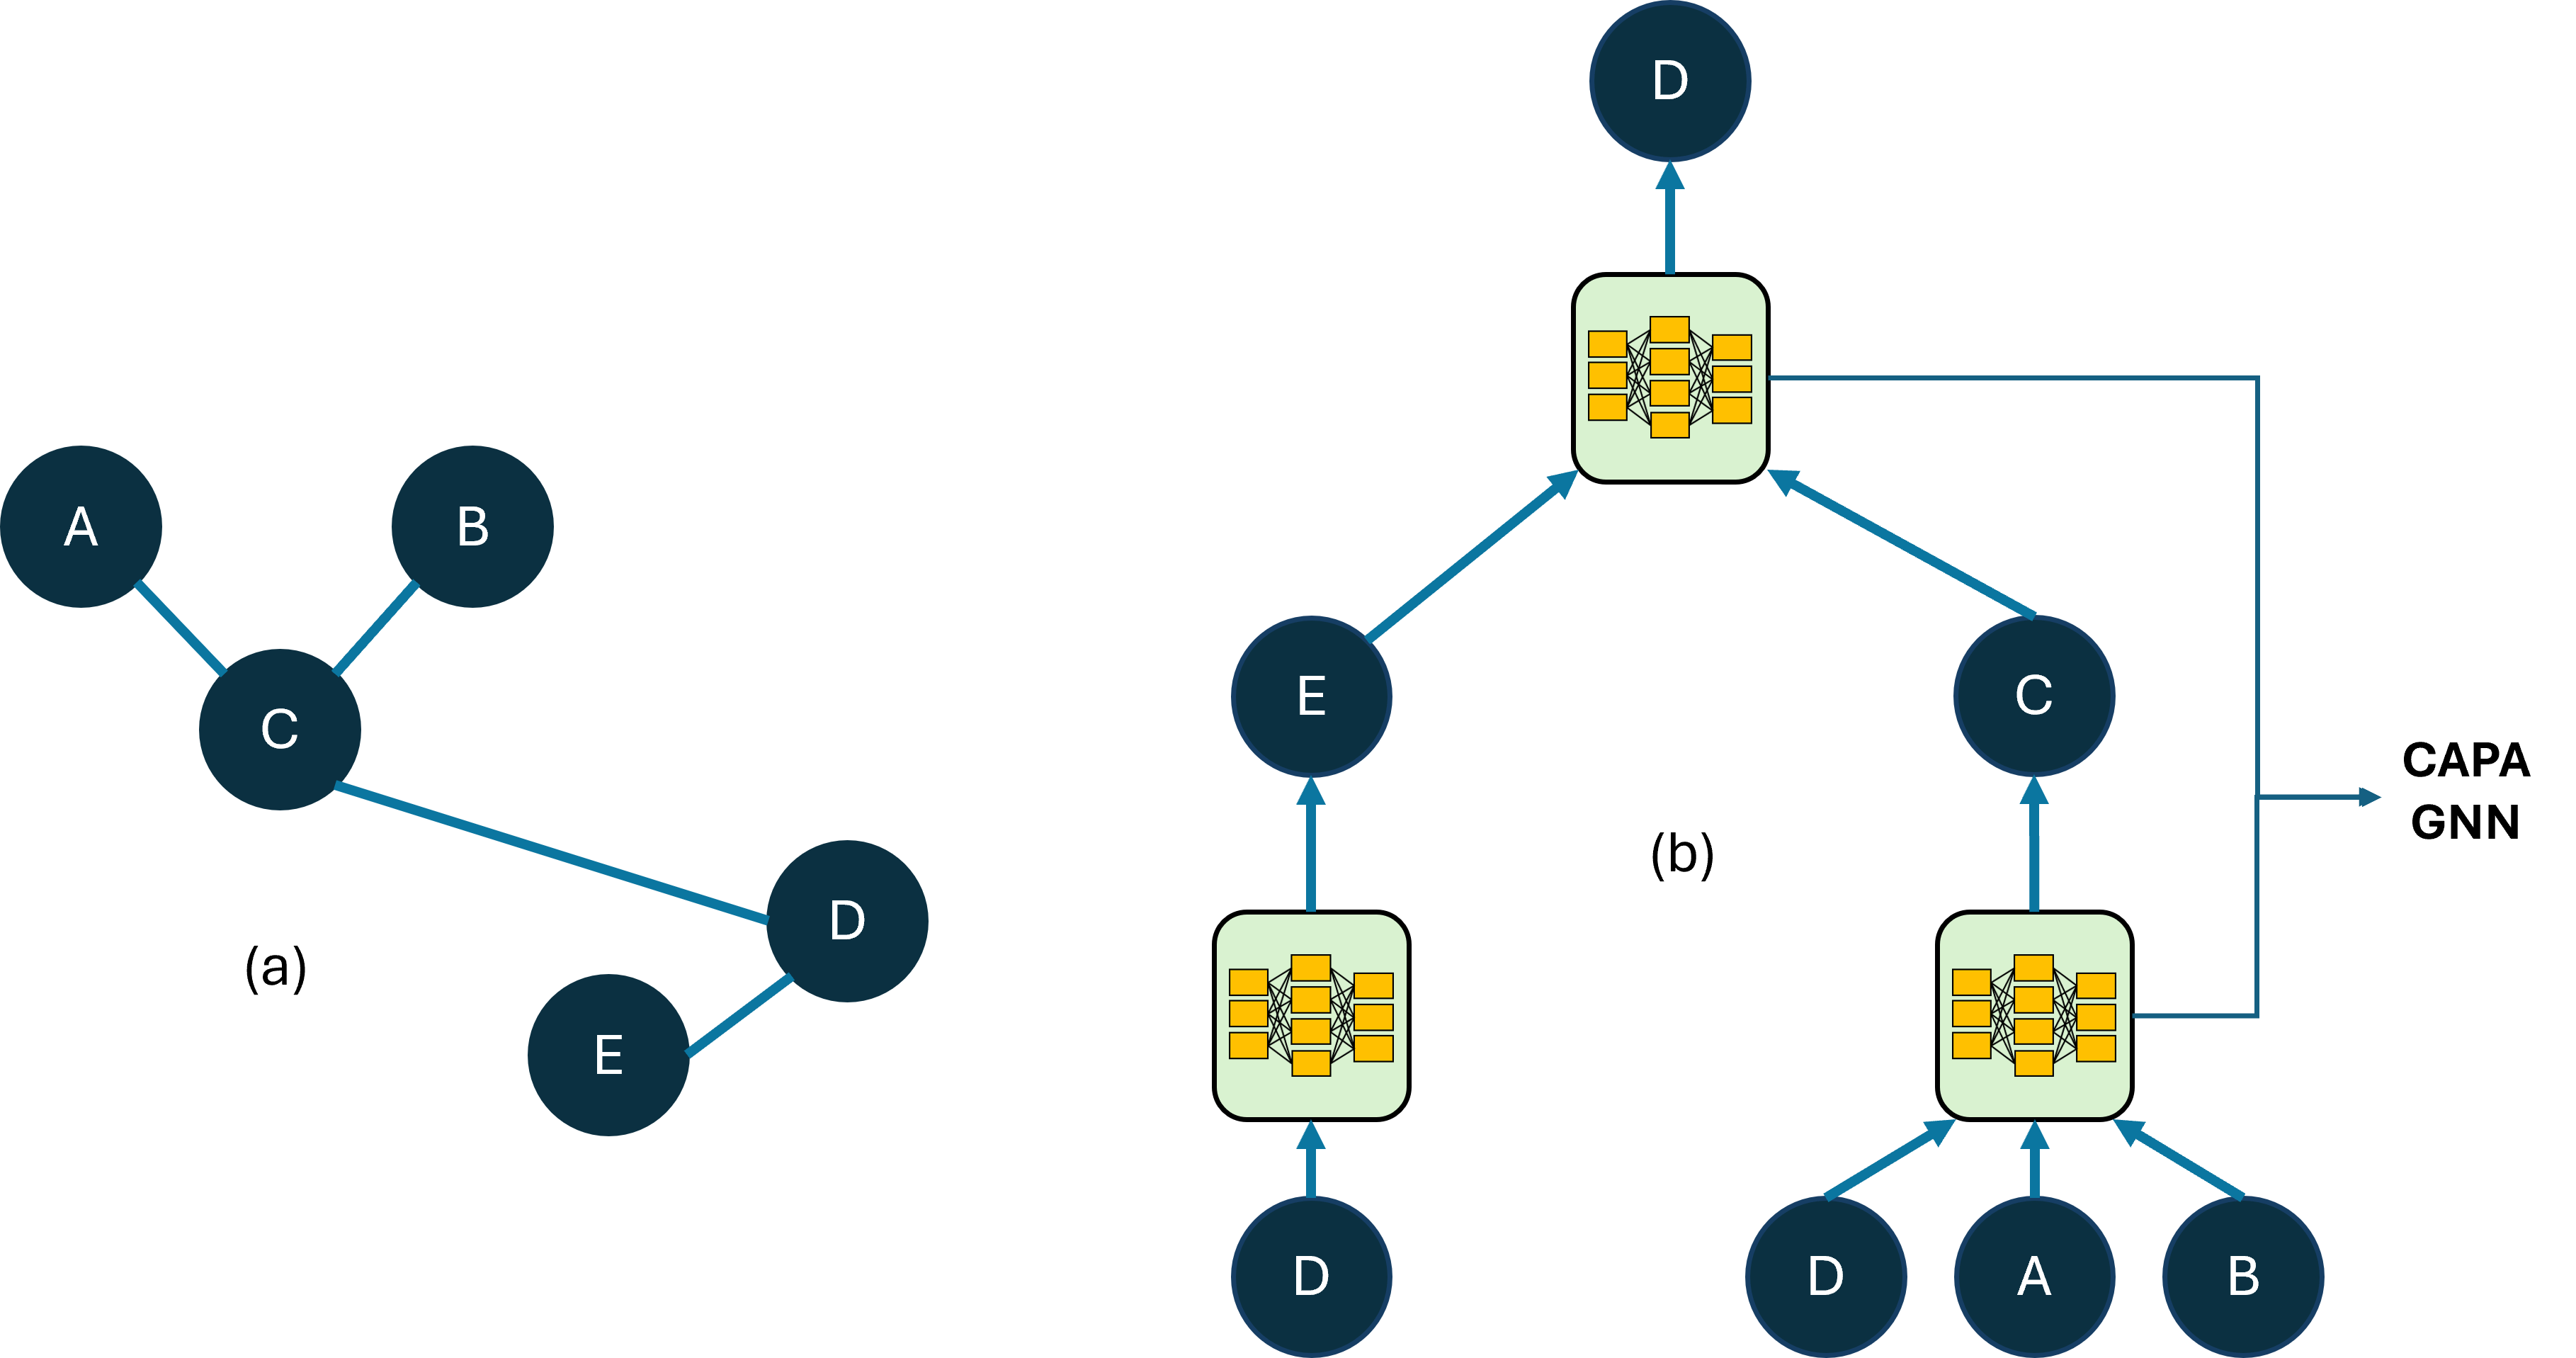
\includegraphics[width=0.9\textwidth]{Imagenes/GNN.png}
    \caption{Ilustración de grafo de entrada (a) y el proceso de la GNN en el cual se realiza el cálculo de la representación vectorial del nodo E agregando información de los nodos vecinos (b).}
    \label{fig:GNN}
\end{figure}

\subsubsection{Grafos}
\subsubsection{GAT}
\subsubsection{GCN}
\subsubsection{GTN}